\section{Verwirklichung der Anforderungen}

\begin{figure}[H]
    \centering
    \caption{system architecture}
    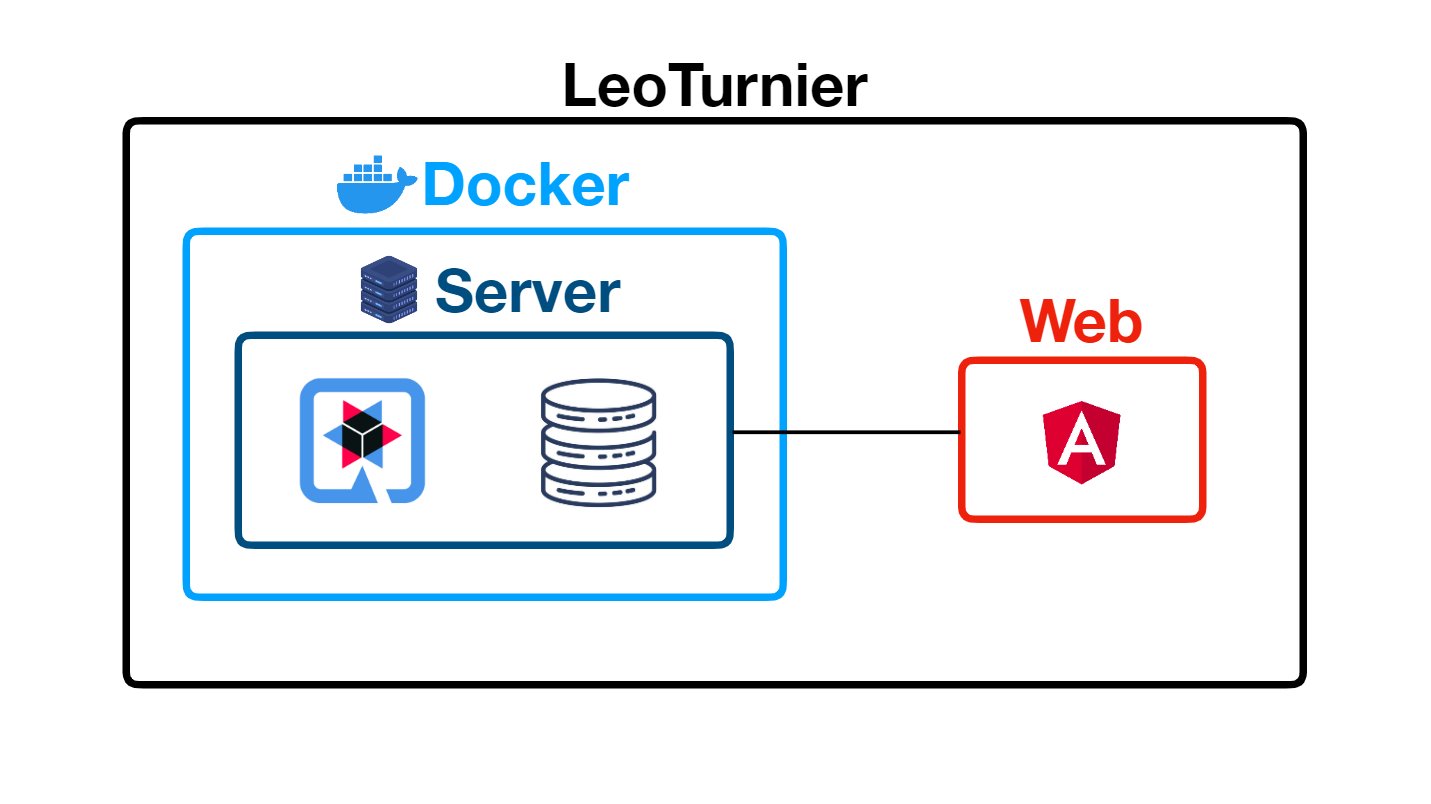
\includegraphics[scale=0.25]{pics/system_architecture.png}
\end{figure}


\section{Verwendete Technologien}

\subsection{Git}

\includegraphics[scale=0.05]{pics/git.png}

Git ist das mit Abstand am weitesten verbreitete Versionskontrollsystem der Welt. Der Name Git wird aus der britischen 
Umgangssprache übersetzt und bedeutet "Blödmann.
\cite{sysarch-git-1}
Es ist ein Open-Source Projekt, 
das ursprünglich 2005 von dem Entwickler des Linux Betriebsystem-Kernels entwickelt wurde. Es ist außerdem mit sowohl mit 
Windows als auch Linux Systemen kompatibel und auch in vielen verschiedenen IDEs integriert. Git ist ein verteiltes Versionskontrollsystem, 
was bedeutet, dass der Versionsverlauf nicht nur an einem Ort gespeichert ist, wie es bei älteren Versionskontrollsystemen der Fall war, 
sondern in jeder Arbeitskopie der gesamte Verlauf aller Änderungen im Repository (Aufbewahrungsort) enthalten sind. 

\cite{sysarch-git-2}

\subsubsection{Was ist ein Versionskontrollsystem?}

Ein Versionskontrollsystem wie Git wird in der Softwareentwicklung verwendet, 
um Änderungen des Quellcodes zu speichern und zu verwalten. 
Hier gibt es drei Arten von Versionskontrollsystemen:
\cite{sysarch-git-2}
\begin{itemize}
 \item lokale Versionsverwaltung (Local Version Control System - LVCS): 
\end{itemize}
Hier werden Dateien lokal einfach nur in ein separates Verzeichnis kopiert.
\cite{sysarch-git-2}
\begin{itemize}
 \item zentrale Versionsverwaltung (Centralized Version Control System - CVCS):
\end{itemize}
Hier gibt es einen einen zentralen Server, der alle versionierten Dateien verwaltet und es Personen ermöglicht, 
Dateien von diesem zentralen Repository abzuholen und auf ihren PC zu übertragen.
\cite{sysarch-git-2}
\begin{itemize}
 \item verteilten Versionsverwaltung (Distributed Version Control System - DVCS):
\end{itemize}
Wie weiter oben schon angesprochen ist diese Variante jene, die von Git benutzt wird. Hier gibt es zwar ein zentrales Repository, 
aber jede Person  hat eine Kopie des Repositories und somit die vollständigen Projektdaten.
\cite{sysarch-git-2}

\subsubsection{Git Befehle}

Git verwendet zum verwalten eines Repositories das Terminal, hierzu gibt es einige wichtige Befehle. Zuerst kann man mit "git init" ein leeres Repository erstellen 
oder ein existierendes nochmal initialisieren, alternativ kann man mit "git clone" ein existierendes Repository kopieren. Damit ein File von Git gespeichert werden
kann, muss man es zunächst mit "git add" zum Repository hinzufügen, das ganze kann dann mit "git rm" wieder rückgängig gemacht werden. Mit "git status" wird der 
momentane Status aller Files im Repository angezeigt, dass heißt, ob das File neu im Repository ist, ob es seit dem letzten Mal Speichern verändert wurde, oder ob es 
erst garnicht im Repository vorhanden ist. Nun kann man mit "git commit" den momentanen Status des Repositories als neue Version speichern und mit "git push" an ein "remote" 
Repository senden. Als letzter wichtiger Befehl gilt noch "git branch", hiermit kann man das Repository in verschiedene "Branches" aufteilen und so 
neue Features getrennt voneinander entwickeln, und diese dann mit "git merge" im Hauptbranch zusammenfügen.
\cite{sysarch-git-2}

\subsection{Github}

\includegraphics[scale=0.05]{pics/github.png}

Github ist ein Cloud-basiertes Repository Hosting Service, das die verteilte Versionskontrolle von Git zur verfügung stellt. Es wurde 2008 von Chris Wanstrath, P. J. Hyett, 
Scott Chacon und Tom Preston-Werner gestartet. Zu dem Zeitpunkt war Git noch relativ unbekannt, wesshalb es noch keine anderen Optionen gab. Die Software wurde in der 
Programmiersprache "Ruby on Rails and Erlang" entwickelt. 
\cite{sysarch-github-1}
Das Ziel von Github ist es, eine benutzerfreundliche Oberfläche für Git zur verfügung zu stellen, mit der man auch mit weniger technischem Wissen die Vorteile von Git ausnutzen kann.
\cite{sysarch-github-2}
Als Unternehmen verdient GitHub Geld, indem es gehostete private Code-Repositories sowie andere geschäftsorientierte Pläne verkauft, 
die es Unternehmen erleichtern, Teammitglieder und Sicherheit zu verwalten.
\cite{sysarch-github-2}

\subsubsection{Github Issues}

Github verfügt über einen integrierten issue tracken, mit dem sich Issues auf GitHub verwalten lassen. Ein Issue ist eine 
Aufgabe im Projekt, die mit dem Titel kurz, und dann in der Beschreibung genauer beschrieben wird, und einem bestimmten Entwickler 
zugeteilt wird. Ein Issue kann den Status "open" oder "closed" haben, "open" bedeutet, dass die Aufgabe noch nicht erfüllt wurde, und 
"closed" bedeutet dass die Aufgabe schon erfüllt ist. Github Issues haben gegenüber von anderen issue trackern vorallem einem Vorteil, 
weil es direkt dort ist, wo auch der Quellcode zu finden ist, jedoch ist es weit nicht so mächtig wie manch andere Optionen, wesshalb 
sich bei dieser Arbeit nicht für Github Issues entschieden wurde.
\cite{sysarch-github-3}

\subsubsection{Github Actions}

GitHub Actions ist ein in Github integriertes Tool, um Prozesse in einem Softwareprojekt zu automatisieren. 
Dadurch kann man Workflows für dein Repository erstellen. Ein Workflow besteht aus einem oder mehreren Jobs, 
wobei ein Job aus einem oder mehreren Schritten besteht. Man kann festlegen, ob Workflows in einem Container oder in einer virtuellen 
Maschine ausgeführt werden sollen. Die Ausführung kann unter den gängigen Betriebssystemen Windows, Linux und macOS erfolgen. 
Workflows werden durch Events wie beispielsweise ein Push auf das Repository ausgelöst und ausgeführt. Wenn ein Workflow ausgeführt wird, 
arbeitet er alle seine Jobs, sowie Schritte ab und erstellt dir ein umfangreiches Feedback mit Logs und Ausführungszeiten. 
Das Feedback kann individuell für jeden Schritt angepasst werden. Eine Action wird in der Web-Oberfläche von GitHub erstellt. 
Praktischerweise kann eine erstellte Action geteilt und wiederverwendet werden.
\cite{sysarch-github-4}

\subsubsection{Github Packages}

Ein Package ist ein wiederverwendbares Stück Software, das von einer globalen Registry in die lokale Umgebung eines Entwicklers heruntergeladen und 
in den Anwendungscode integriert werden kann. Da Pakete als wiederverwendbare "Bausteine" fungieren und in der Regel allgemeine Anforderungen erfüllen 
(z. B. API-Fehlerbehandlung), können sie zur Verkürzung der Entwicklungszeit beitragen. Github Packages ist ein Package Managing Service, 
der die Veröffentlichung von Packages erleichtert und vollständig in GitHub integriert ist. Alles befindet sich an einem Ort, 
sodass man zum Suchen und Veröffentlichen von Paketen dieselben Such-, Browsing- und Verwaltungstools verwenden kann wie für Repositories.
\cite{sysarch-github-5}

\subsection{Intellij IDEA}

\includegraphics[scale=0.05]{pics/intellijIdeaLogo.png}

IntelliJ IDEA ist eine intelligente, kontextsensitive IDE für Java und andere JVM-Sprachen wie Kotlin, Scala und Groovy, die sich für zahlreiche 
Anwendungsbereiche eignet. Auch bei der Entwicklung von Full-Stack-Webanwendungen hilft IntelliJ IDEA Ultimate mit integrierten Tools, 
Unterstützung für JavaScript und verwandte Technologien sowie erweiterte Unterstützung für gängige Frameworks wie Spring, Spring Boot, Jakarta EE, Micronaut, 
Quarkus oder Helidon. Darüber hinaus kann IntelliJ IDEA mit Plugins von JetBrains erweitern, um die IDE mit anderen Programmiersprachen wie 
Go, Python, SQL, Ruby und PHP einzusetzen. 
\cite{sysarch-intellij-1}

\subsubsection{Was ist eine IDE?}

Eine IDE (Integrated Development Environment) oder integrierte Entwicklungsumgebung ist Software für die Anwendungsentwicklung, 
die gängige Entwicklertools in einer zentralen grafischen Oberfläche vereint. Eine typische IDE besteht aus folgenden Komponenten:
\cite{sysarch-intellij-2}
\begin{itemize}
 \item Quellcode-Editor 
\end{itemize}
Ein Texteditor, der eine Programmierung von Software-Code mit folgenden Features unterstützt: 
Syntaxhervorhebung mit visuellen Hinweisen, sprachspezifische Autovervollständigung und eine Bug-Prüfung, während der Code geschrieben wird.
\cite{sysarch-intellij-2}
\begin{itemize}
 \item Automatisierung lokaler Builds
\end{itemize}
Dienstprogramme, mit denen sich einfache wiederholbare Aufgaben im Rahmen der Entwicklung lokaler Software-Builds zur Nutzung durch 
die Entwickler automatisieren lassen, wie beispielsweise die Kompilierung von Quell- in Binärcode, dessen Paketierung und die Ausführung automatischer Tests.
\cite{sysarch-intellij-2}
\begin{itemize}
 \item Debugger
\end{itemize}
Ein Programm zur Prüfung anderer Programme, mit dem sich die Position von Bugs im Originalcode grafisch anzeigen lässt.
\cite{sysarch-intellij-2}


\subsubsection{Codeanalyse}

Intellij bietet intelligente Programmierhilfen an. Durch eine Indizierung des Quellcodes legt die IDE eine virtuelle 
Karte des Projekts an. Anhand der Informationen in dieser virtuellen Karte kann sie Fehler erkennen, kontextabhängige Completion-Vorschläge anbieten oder
Refactorings durchführen.
\cite{sysarch-intellij-1}


\subsubsection{Versionsverwaltung}

IntelliJ IDEA unterstützt die gängigen Versionsverwaltungen (VCS) wie Git, Subversion, Mercurial und Perforce. 
Man kann ein VCS-Projekt direkt auf dem Startbildschirm klonen, die Unterschiede zwischen zwei Revisionen untersuchen, Branches verwalten, 
Commits durchführen und pushen, Konflikte bereinigen oder den Verlauf überprüfen. 
\cite{sysarch-intellij-1}


\subsubsection{JVM-Frameworks}

IntelliJ IDEA Ultimate bietet Unterstützung für Frameworks und Technologien zur Entwicklung von Anwendungen und Microservices. 
Die IDE bietet spezielle Unterstützung unter anderem für Quarkus, Spring, Spring Boot, Jakarta EE, JPA und Reactor.
\cite{sysarch-intellij-1}


\subsection{WebStorm}
\includegraphics[scale=0.025]{pics/WebStormLogo.svg.png}


Obwohl es möglich wäre mit Intellij ein Angular Projekt zu entwickeln haben wir uns bei der Frontend Entwicklung 
für die IDE Webstorm entschieden. Diese ist genauso wie Intellij von Jetbrains doch enthält mehr support für die 
Programmiersprachen JavaScript und TypeScript, sowie einen Built-in Debugger für Client-Side JavaScript und Node.js 

\subsection{Quarkus}

\includegraphics[scale=0.015]{pics/quarkusLogo.png}

Quarkus ist ein Framework zur Erstellung von Java-Anwendungen mit dem Java speziell für Container optimiert wird. 
Es bietet eine effektive Plattform für Serverless-, Cloud- und Kubernetes Umgebungen. Der Hersteller Redhat wirbt 
auch mit schnellen Startzeiten und geringen Speicherplatzverbrauch. Dise erzielt Quarkus dadurch dass es den Code schon Buildvorgangs verabeitet.

\subsection{Maven}

\includegraphics[scale=0.015]{pics/apacheMavenLogo.svg.png}

Maven ist ein Build Atomation Tool welches hauptsächlich für Java verwendet wird und folgt dem Ansatz Konvention vor Konfiguration. TODO


\subsection{Angular}

\includegraphics[scale=0.02]{pics/angularLogo.svg.png}

Angular ist ein Client-Side JavaScript Framework zur Erstellung von Single-Page-Webapplications. 
Seine komponentenbasierte Architektur welche View und Logik trennt macht es für den Entwickler leicht 
Applikationen zu warten und testen. Dabei verwendet Angular TypeScript für den Code-Behind und HTML als Auszeichnungssprache. 
Die vielen gut integrierten Libraries decken Features wie Routing, Verwaltung von Formulare und Client-Server Kommunikation ab. 

\subsection{PostgreSQL}

\includegraphics[scale=0.015]{pics/postgresqlLogo.svg.png}

PostgreSQL ist eine objektrelationale Datenbank welche sich durch ihre Stabilität und freie Verfügbarkeit auszeichnet. 
Sie hält sich dabei sehr eng an den SQL-Standard. Es werden eine Vielzahl von Datentypen und Operatorn unterstützt und 
Entwickler können auch eigene Datentypen definieren. Ein weitetere großer Vorteil von PostgreSQL ist auch dass es auf 
jeder Hardware und auf beinahe jedem Betriebsystem läuft. 
\subsection{Docker}
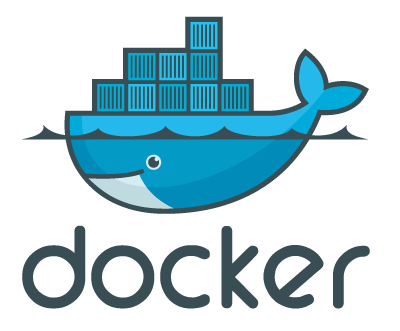
\includegraphics[scale=0.05]{pics/dockerLogo.png}

Docker ist eine Software zur Containervirtualisierung . Die Container sind voneinander isoliert und haben ihre eigene Software, 
Libraries sowie Konfigurationsdatein. Kommunizieren können sie über vorher genau definierte Kanäle. Da alle Container 
auf dem selben OS-Kernel laufen brauchen sie weniger Resourcen wie eine Virtuele Maschine.